\chapter{Desenvolvimento do Projeto}
\label{chap:resultados}

    A etapa de desenvolvimento do projeto desempenha um papel abrangente, contudo, extremamente crucial para a transformação de ideias em aplicações práticas, como definição do escopo do projeto, histórias de usuários, requisitos funcionais e não funcionais, definição de tecnologias e estabelecimento da arquitetura do modelo. Um estabelecimento robusto desses aspectos, ainda na etapa inicial do desenvolvimento, evita conflitos de requisitos no futuro ou impossibilidade de implementação do projeto devido à falta de clareza no escopo do projeto.   

\section{Escopo do Projeto}
\label{sec:resultados-do-experimento-a}

    A bengala inteligente é uma ferramenta de TA que busca auxiliar usuários com deficiência visual a se locomover com mais independência e autonomia pelo espaço. O acoplamento de um microcontrolador e diferentes sensores na bengala fornecem ao usuário uma maior noção do ambiente, a fim de devolver capacidades funcionais prejudicadas no campo da visão.

    \subsection{O que a bengala inteligente é?}
        \begin{itemize} 
            \item Uma ferramenta de assistência para pessoas com deficiência visual, projetada para melhorar a mobilidade e a independência.
            
            \item Capaz de detectar obstáculos sólidos e outros elementos do ambiente que possam representar riscos à segurança.
            
            \item Equipada com sensores que fornecem feedback tátil ou auditivo ao usuário, permitindo uma navegação mais eficiente e segura.
            
            \item Projetada para ser leve, fácil de usar e confortável durante o uso prolongado.
            
            \item Voltada para garantir uma longa duração da bateria.
        \end{itemize}

\section{Requisitos Funcionais}
    Requisitos funcionais em sistemas embarcados definem as funcionalidades específicas que o sistema deve realizar, levando em conta as limitações de recursos do hardware. Dessa forma, estabelece as funcionalidades que a bengala fornece ao usuário e como o processamento de dados captados por sensores devem ser tratados.


\begin{table}[!ht]    
    \captionsetup{width=1.0\textwidth} % Definindo a largura da legenda
    \caption{Requisitos funcionais da bengala inteligente}  
    \renewcommand{\arraystretch}{1.5} % Aumenta o espaçamento entre as linhas
    \begin{tabular}{p{0.1\textwidth}p{0.2\textwidth}p{0.6\textwidth}} % Definindo larguras para as colunas
        \toprule
        Referência & Nome & Descrição \\
        RF01 & Identificação de objetos & A bengala deve ser capaz de detectar objetos sólidos, como paredes, móveis ou obstáculos, a uma distância de pelo menos um metro em relação aos sensores.   \\
        RF02 & Altura de objetos  & A bengala deve conseguir identificar objetos em diferentes alturas, desde o solo até o peito. \\
        RF03 & Detecção em ambientes escuros  &  A bengala deve ser capaz de identificar objetos independentemente da iluminação do local.  \\
        RF04 & Modo de vibração  &  A intensidade da vibração deve variar de acordo com a distância do objeto identificado, de forma que a vibração aumente conforme a distância diminui.  \\
        RF05 & Diferença entre os modos de vibração  & A alternância de intensidade deve ser perceptível ao usuário. \\
        RF06 & Recarregamento da bengala  & A bengala deve ser recarregável.  \\
        RF07 & Indicador de carga completa  &  Deve existir um sinal sonoro na bengala para indicar que a bateria foi completamente recarregada.  \\
        RF08 & Desligamento  & A bengala deve possuir um interruptor/botão para que seja desligada. \\
        RF09 & Indicador de desligamento  &  Deve existir um sinal sonoro na bengala para indicar que a bengala foi desligada.  \\
        RF10 & Alarme sonoro para caso de perda  &  A bengala deve possuir um sensor touch no apoio de mão que, ao não reconhecer mais toque durante um certo período de tempo, ative um alarme sonoro para alertar o usuário acerca da localização.  \\
        \bottomrule
    \end{tabular}
    \caption*{Fonte: elaborada pelos autores.} % Legenda sem rótulo
\end{table}


\section{Requisitos Não Funcionais}
    Os requisitos não funcionais se concentram em qualidades do sistema além das funcionalidades diretas. Isso pode incluir restrições de desempenho, consumo de energia pela bengala, latência de resposta, especificações técnicas, compatibilidade entre componentes e tamanho do conjunto de hardware.


\begin{table}[!ht]    
    \captionsetup{width=1.0\textwidth} % Definindo a largura da legenda
    \caption{Requisitos não funcionais da bengala inteligente}  
    \renewcommand{\arraystretch}{1.5} % Aumenta o espaçamento entre as linhas
    \begin{tabular}{p{0.1\textwidth}p{0.2\textwidth}p{0.6\textwidth}} % Definindo larguras para as colunas
        \toprule
        Referência & Nome & Descrição \\
        RNF01 & Tempo de vibração & O tempo entre a detecção de um objeto e o alarme através do motor de vibração não pode ser superior a um segundo.   \\
        RNF02 & Tempo de detecção  & A detecção dos objetos deve ocorrer em tempo real. \\
        RNF03 & Precisão  &  A identificação de objetos deve ser precisa e confiável, sem falsos positivos ou negativos.  \\
        RNF04 & Integração ergonômica  &  Os componentes e módulos devem ser integrados na bengala de forma discreta.  \\
        RNF05 & Entrada do carregador  & A entrada para recarregar a bengala deve ser do tipo micro USB. \\
        RNF06 & Proteção contra sobrecarga  & A recarga não deve oferecer riscos à bateria ou ao usuário, devendo existir uma proteção contra superaquecimento ou sobrecarga.  \\
        RNF07 & Autonomia de bateria  &  A bateria deve durar, no mínimo, 8 horas entre cada recarga. \\
        RNF08 & Resistência da entrada  & A entrada do carregador deve ser resistente e fixa na estrutura da bengala. \\
        RNF09 & Conforto  &  A bengala deve possuir apoio de mão e ponteira.  \\
        RNF10 & Distribuição do peso &  O peso da bengala deve ser distribuído ao longo da extensão ou estar concentrado próximo ao apoio de mão.  \\
        RNF11 & Informações na bengala &  Todas as informações, como o indicador de ligado/desligado, devem estar escritas em Braille.  \\
        \bottomrule
    \end{tabular}
    \caption*{Fonte: elaborada pelos autores.} % Legenda sem rótulo
\end{table}

\section{Histórias de usuário}

    Histórias de usuário são projetadas para capturar requisitos de forma simples e compreensível. Cada história de usuário descreve uma funcionalidade do sistema do ponto de vista do usuário final, fornecendo contexto sobre o que precisa ser feito e por que é importante. Essas histórias são essenciais para manter o foco nas necessidades dos usuários durante todo o ciclo de desenvolvimento, ajudando a equipe a priorizar e planejar suas atividades de forma eficaz. Ao descrever os requisitos em termos de histórias de usuário, as equipes podem garantir que estão construindo as funcionalidades certas para satisfazer as necessidades reais dos usuários finais.
    
    O processo de desenvolver as histórias permite que a equipe possa visualizar os requisitos em termos práticos. Ademais, a elaboração de critérios de aceitação para cada requisito auxilia o processo de teste e validação das funcionalidades, uma vez que define em termos práticos o que deve ser alcançado para que o desenvolvimento seja considerado bem-sucedido.

    \subsection{Recarregamento da Bengala}
    \begin{quote}
    \textit{Como usuário, preciso que recarregar a bengala seja um processo simples e conveniente, garantindo sua prontidão para uso sempre que necessário e evitando que fique inutilizada devido à falta de carga.}
    \end{quote}    
    \noindent\textbf{Critérios de Aceitação:}
    \begin{itemize}
        \item O processo de recarga deve ser simples e intuitivo, exigindo apenas uma conexão fácil entre a bengala e a fonte de energia, como um cabo USB ou um adaptador de energia.
        \item A bengala deve possuir uma entrada para um cabo simples de ser encontrado no mercado, como micro USB, USB-C ou USB.
        \item Deve haver um indicador sonoro que informe ao usuário quando a bateria estiver completamente carregada, para garantir que o processo de recarga seja concluído com sucesso.
        \item O tempo necessário para recarregar a bateria da bengala deve ser razoável e adequado para o uso diário, evitando longos períodos de espera para que o dispositivo esteja pronto para uso novamente.
        \item O conector da bengala deve ser resistente, a fim que suporte múltiplas conexões e desconexões ao longo do tempo sem entortar, quebrar, afundar ou parar de funcionar.
        \item O processo de recarga deve ser seguro e protegido contra sobrecarga, curto-circuito ou superaquecimento, para evitar danos à bateria ou riscos para o usuário durante o carregamento.
        \item A bateria da bengala deve ter autonomia e durar, ao menos, 8 horas entre cada recarga.
    \end{itemize}

    \subsection{Resposta tátil}
    \begin{quote}
    \textit{Como usuário, desejo que a vibração da bengala forneça uma resposta tátil que indique a distância dos objetos dos quais estou me aproximando.}
    \end{quote}    
    \noindent\textbf{Critérios de Aceitação:}
    \begin{itemize}
        \item Quando um objeto estiver a uma distância segura, a vibração da bengala deve ser suave e contínua.
        \item À medida que o usuário se aproxima de um objeto, a intensidade ou frequência da vibração deve aumentar gradualmente, indicando a proximidade.
        \item Quando o usuário estiver a uma distância perigosa ou muito próxima do objeto, a vibração deve ser forte e intermitente, alertando-o para uma possível colisão.
        \item A resposta tátil da bengala deve ser clara e compreensível, permitindo que o usuário interprete facilmente a distância dos objetos ao seu redor.
    \end{itemize}
        
    \subsection{Detecção de objetos}
    \begin{quote}
    \textit{Como usuário, preciso que a bengala possa identificar objetos à frente para que eu permaneça seguro.}
    \end{quote}    
    \noindent\textbf{Critérios de Aceitação:}
    \begin{itemize}
        \item A bengala deve ser capaz de detectar objetos sólidos, como paredes, móveis ou obstáculos, a uma distância segura de pelo menos um metro à frente do usuário.
        \item A bengala deve conseguir identificar objetos em diferentes alturas.
        \item A identificação de objetos deve ser precisa e confiável, evitando falsos positivos ou negativos.
        \item Quando um objeto for detectado, a bengala deve fornecer um alerta imediato ao usuário, seja por meio de vibração, som ou outro meio de feedback sensorial.
        \item A detecção de objetos deve ocorrer em tempo real, permitindo que o usuário reaja rapidamente para evitar colisões ou acidentes.
        \item A bengala deve ser capaz de identificar objetos em diferentes condições de iluminação, garantindo sua eficácia tanto durante o dia quanto à noite.
        \item O sistema de identificação de objetos deve ser integrado de forma discreta e ergonômica à bengala, sem comprometer sua funcionalidade ou conforto para o usuário.
    \end{itemize}

    \subsection{Resistência à água}
    \begin{quote}
    \textit{Como usuário, gostaria que a bengala fosse resistente à água para que eu possa sair com ela mesmo com chuva.}
    \end{quote}    
    \noindent\textbf{Critérios de Aceitação:}
    \begin{itemize}
        \item Os materiais utilizados para construir a bengala devem ser resistentes à água e que não absorvam umidade.
        \item Os componentes elétricos (incluindo microcontrolador, componentes e fios) devem estar armazenados em um recipiente vedado.
    \end{itemize}
        
    \subsection{Portabilidade}
    \begin{quote}
    \textit{Como usuário, gostaria que a bengala fosse leve e fácil de usar, para que não seja exaustivo manter o uso por um longo período de tempo.}
    \end{quote}    
    \noindent\textbf{Critérios de Aceitação:}
    \begin{itemize}
        \item A bengala deve possuir dimensões similares às de outras bengalas encontradas no mercado.
        \item A bengala deve ser leve o suficiente para que não seja cansativo utilizá-la e mantê-la inclinada durante o uso.
    \end{itemize}
                
    \subsection{Desligar circuito}
    \begin{quote}
    \textit{Como usuário, desejo poder desligar a bengala para que não permaneça desnecessariamente ligada enquanto não estiver sendo utilizada.}
    \end{quote}    
    \noindent\textbf{Critérios de Aceitação:}
    \begin{itemize}
        \item A bengala deve possuir um mecanismo de desligamento fácil, como um interruptor físico ou um botão de desligamento.
        \item O botão ou interruptor de desligamento deve ser mapeado na bengala de forma tátil, utilizando braille ou outra indicação tátil.
        \item Quando desligada, a bengala não deve consumir energia da bateria para garantir uma vida útil prolongada da mesma.
        \item O desligamento da bengala deve ser confirmado por meio de um indicador sonoro para garantir que o usuário saiba quando a bengala está realmente desligada.
        \item O processo de ligar e desligar a bengala deve ser rápido e conveniente, sem a necessidade de procedimentos complicados ou demorados.
        \item O mecanismo de desligamento deve ser robusto e confiável, com um design que evite desligamentos acidentais durante o uso normal da bengala.
        \item O desligamento da bengala não deve afetar negativamente outras funcionalidades ou operações da mesma, garantindo uma transição suave entre os estados ligado e desligado.
    \end{itemize}
                        
    \subsection{Conforto}
    \begin{quote}
    \textit{Como usuário, preciso que a bengala seja confortável durante o uso de forma que os componentes eletrônicos adicionais não a tornem mais desconfortável que uma bengala analógica comum.}
    \end{quote}    
    \noindent\textbf{Critérios de Aceitação:}
    \begin{itemize}
        \item O peso da bengala deve ser distribuído ao longo da extensão ou estar concentrado próximo à mão do usuário, para que não exija muito torque durante a utilização.
        \item A bengala deve possuir apoio de mão e ponteira.
        \item A adição dos componentes não pode ocupar um espaço excessivo no corpo da bengala.
    \end{itemize}

    \section{Componentes}
    É fundamental considerar uma variedade de fatores ao escolher os elementos que comporão o projeto. Além da disponibilidade das peças no mercado, é essencial avaliar o valor e o desempenho de cada componente dentro do propósito funcional da bengala. 

    \subsection{Módulo Motor de vibração}
    O motor de vibração está integrado a um módulo que conta com dois pinos de alimentação e um de entrada. Esse design permite que o módulo receba uma tensão variável, ajustando assim a intensidade da resposta vibratória do motor conforme necessário.

    Com capacidade para alcançar até 9000 rotações por minuto (RPM), o motor é responsável por gerar a sensação de vibração percebida pelo usuário. Essa característica torna o módulo ideal para controlar a resposta tátil do usuário com base na detecção de obstáculos próximos.
    
    A operação do módulo é simples: ele recebe uma tensão de até 5V na porta digital para ativar o motor. Além disso, é possível controlar a frequência da vibração por meio do envio de pulsos rápidos para o módulo pela porta digital.
    
     \begin{figure}[h!]
        \captionsetup{width=1\textwidth}
        \caption{\label{fig:motorvibracao} Módulo do motor de vibração}
        \centering
        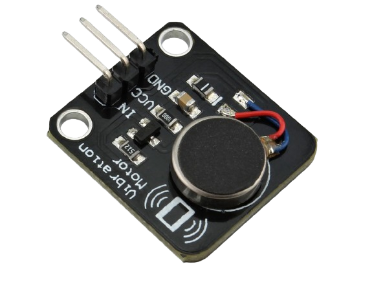
\includegraphics[width=0.3\textwidth]{figuras/motorvibracao} 
        \caption*{Fonte: Mercado Livre}
    \end{figure}

    \subsection{Módulo Sensor de Distância Ultrassônico HC-SR04}

    O sensor ultrassônico, parte integrante da bengala inteligente, desempenha uma função essencial ao detectar a distância entre o usuário e os objetos circundantes. Essa capacidade permite fornecer um feedback preciso sobre a localização e proximidade dos obstáculos. Este modelo de sensor destaca-se pela sua acessibilidade e possui um alcance efetivo de até quatro metros de distância em relação aos objetos detectados.

     \begin{figure}[ht]
        \captionsetup{width=1\textwidth}
        \caption{\label{fig:hcsr04} Módulo Sensor de Distância Ultrassônico HC-SR04}
        \centering
        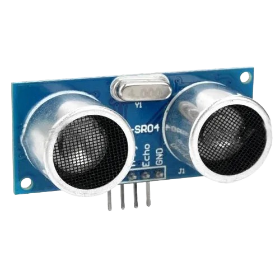
\includegraphics[width=0.3\textwidth]{figuras/hcsr04} 
        \caption*{Fonte: RoboCore}
    \end{figure}


    \subsection{Sensor Capacitivo Touch TTP223B}

    O sensor capacitivo touch, localizado na área de aderência da bengala inteligente, oferece uma interação intuitiva para o usuário. Ao detectar o toque, a bengala permanece no mesmo estado normal de funcionamento, detectando obstáculos e vibrando. No entanto, caso o sensor não detecte nenhum toque por um período determinado, ele ativará um alarme sonoro, permitindo que o usuário encontre a bengala ou a desligue caso tenha sido deixada ligada inadvertidamente.

    Sensores de toque funcionam como uma chave, de forma que ativem um circuito elétrico e permitam o fluxo da corrente caso algum toque seja identificado. 
    
    Sensores capacitivos suportam múltiplos toques em sua região de contato e não exigem pressão aplicada para a a detecção do toque, similar às telas de dispositivos móveis. Dessa maneira, são ideais para o propósito de apenas identificar se existe presença da mão humana.

     \begin{figure}[h!]
        \captionsetup{width=1\textwidth}
        \caption{\label{fig:touch}Sensor Capacitivo Touch TTP223B}
        \centering
        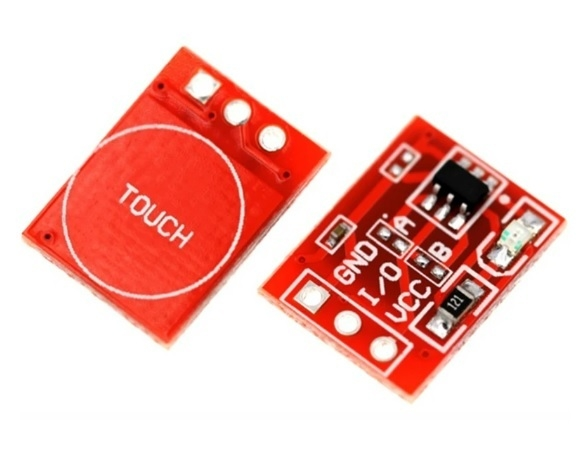
\includegraphics[width=0.3\textwidth]{figuras/touch} 
        \caption*{Fonte: Mercado Livre}
    \end{figure}

    \subsection{Chave DIP Switch}
    O componente Chave DIP Switch 1 Via é responsável por controlar as funcionalidades da bengala inteligente, permitindo ao usuário ligar e desligar os recursos de acordo com suas necessidades. Com a simples alteração da posição da chave, é possível ativar ou desativar as funções da bengala de forma conveniente.

    É um componente que controla o circuito de forma fácil e de baixo custo, além de se adequar melhor ao projeto em relação a um botão por conta da possibilidade de identificar, pelo toque, se a chave está na posição ligada ou desligada.

    \begin{figure}[h!]
        \captionsetup{width=1\textwidth}
        \caption{\label{fig:chave}Chave DIP Switch 1 Via}
        \centering
        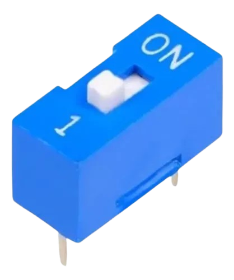
\includegraphics[width=0.3\textwidth]{figuras/chave} 
        \caption*{Fonte: Eletronik LV}
    \end{figure}

    \subsection{Módulo Buzzer Ativo}
    O buzzer ativo desempenha um papel crucial na bengala inteligente ao ser o componente responsável pela emissão sonora, importante como meio de resposta ao usuário com algum grau de deficiência visual. Ele fornece alertas ao usuário quando o sensor de toque não recebe sinais após algum tempo, aprimorando a experiência de uso com a bengala. Seu som nítido e audível garante que informações importantes sejam transmitidas de forma clara e eficaz.

    A preferência ao buzzer ativo justifica-se pela simplicidade de uso e pela ausência de necessidade de emitir diferentes frequências. Similar ao som emitido por microondas, a resposta do buzzer ativo acontece quando o módulo é energizado com uma tensão de até 5V. Dessa forma, não existe a necessidade de especificar o seu funcionamento de forma detalhada no código. 

       \begin{figure}[h!]
        \captionsetup{width=1\textwidth}
        \caption{\label{fig:buzzer}Módulo Buzzer Ativo}
        \centering
        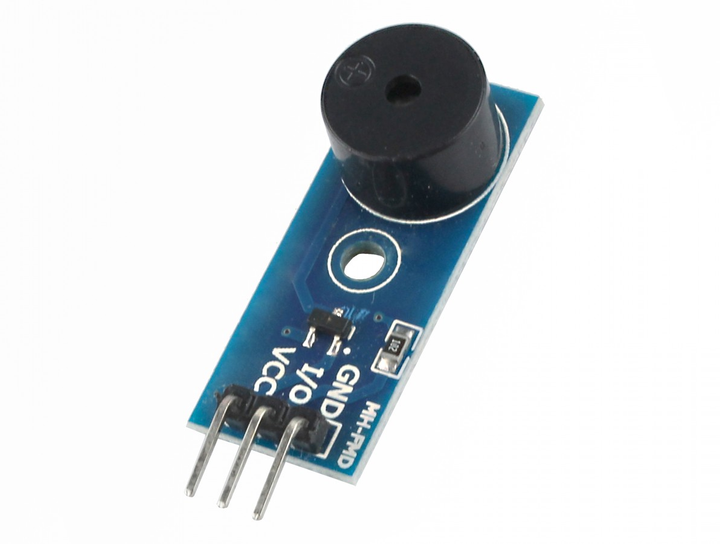
\includegraphics[width=0.6\textwidth]{figuras/buzzer} 
        \caption*{Fonte: A2 Robotics}
    \end{figure}

    \subsection{Protoboard}
    A protoboard é um elemento fundamental na construção da bengala inteligente, oferecendo um ambiente flexível e seguro para a conexão dos componentes eletrônicos. Com sua matriz de furos e trilhas condutoras, a protoboard permite a prototipagem e teste dos circuitos de forma prática e versátil, sem necessidade de soldagem. É nesse espaço que os componentes são interligados e ajustados, proporcionando um ambiente propício para o desenvolvimento e aprimoramento da bengala inteligente.

    \begin{figure}[h!]
        \captionsetup{width=1\textwidth}
        \caption{\label{fig:protoboard} Protoboard de 400 furos}
        \centering
        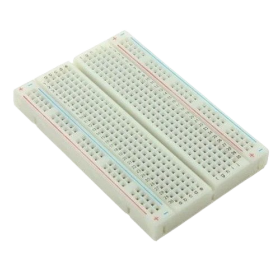
\includegraphics[width=0.3\textwidth]{figuras/protoboard} 
        \caption*{Fonte: Mercado Livre}
    \end{figure}

    \subsection{Microcontrolador}
    A placa Uno R3 é o componente-chave da bengala inteligente, responsável pelo controle e processamento das funcionalidades do dispositivo. É uma peça fundamental para que os sensores consigam ser gerenciados de maneira eficiente. 

    O modelo Uno é equipado com várias portas digitais e analógicas, além de possuir um tamanho compacto, facilitando a montagem de circuitos com integração de diferentes módulos.

    \begin{figure}[h!]
        \captionsetup{width=1\textwidth}
        \caption{\label{fig:arduino} Arduino Uno R3}
        \centering
        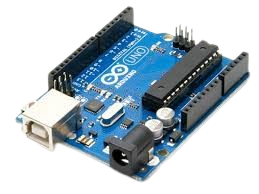
\includegraphics[width=0.3\textwidth]{figuras/arduino} 
        \caption*{Fonte: Fábrica de Bolso}
    \end{figure}

    \subsection{Módulo de Carregamento CN3065}
    Este módulo permite o carregamento de baterias Li-Íon ou Li-Po através de energia solar ou corrente elétrica  com um conector micro USB. Além disso, permite que a bateria possa energizar o microcontrolador de forma segura, uma vez que possui proteção contra sobrecarga e superaquecimento.
    
    \begin{figure}[h!]
        \captionsetup{width=1\textwidth}
        \caption{\label{fig:cn3065} Módulo CN3065}
        \centering
        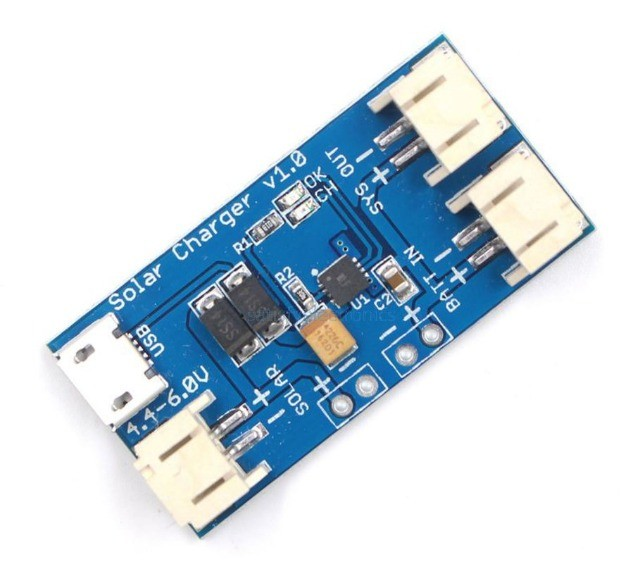
\includegraphics[width=0.3\textwidth]{figuras/cn3065} 
        \caption*{Fonte: AliExpress}
    \end{figure}

    \subsection{Bateria Li-Íon 3,7V 5200mAh}
    A escolha da bateria foi feita considerando o tempo de uso da bateria, dado a corrente elétrica exigida pelos componentes, quanto pela compatibilidade com o módulo de carregamento. Assim, a bateria pode durar bastante tempo e, ainda, energizar todos os módulos do circuito.

     \begin{figure}[h!]
        \captionsetup{width=1\textwidth}
        \caption{\label{fig:bateria}Bateria Li-Íon 3,7V 5200mAh}
        \centering
        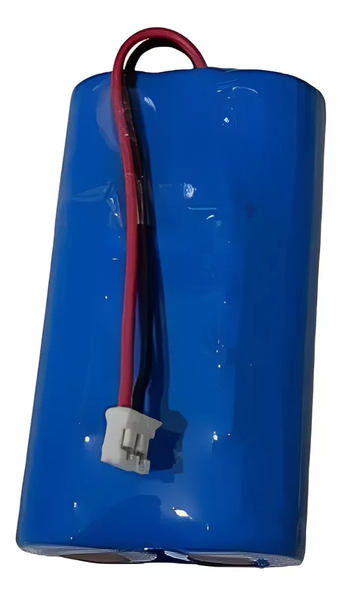
\includegraphics[width=0.2\textwidth]{figuras/bateria} 
        \caption*{Fonte: Mercado Livre}
    \end{figure}

    \section{Viabilidade Financeira}
    O sucesso de um projeto social não se mede apenas pelo impacto que ele gera na comunidade-alvo, mas também pela sua capacidade de se manter ao longo do tempo, sem depender exclusivamente do financiamento dos fundadores. Nesse contexto, a viabilidade financeira de nosso projeto assume um papel fundamental, pois buscamos criar um modelo sustentável que permita a continuidade das atividades sem gerar despesas ou desperdícios.

    Logo, é de suma importância analisar o valor mínimo para a criação da bengala, considerando inicialmente o custo dos materiais, para nortear as possíveis formas de expansão da bengala para o público alvo.

    Primeiramente, é importante destacar que o frete não foi incluído nos custos de produção devido à existência prévia de algumas peças, as quais não tiveram seus preços para entrega registrados. Ainda assim, esses componentes foram incluídos na relação de valores para compra das peças. 

    Além disso, o tempo desempenhou um papel crucial na construção do projeto. Dada a importância de iniciar os testes e cumprir os prazos estabelecidos, priorizamos a compra dos materiais na mesma loja, buscando adquirir a maior quantidade possível de itens em um único local. Essa abordagem não apenas reduziu o tempo de entrega, mas também nos permitiu garantir que todos os componentes chegassem juntos, facilitando o início das atividades de teste.

    Para um projeto em escala real, a aquisição de itens em grande quantidade e a diversificação dos fornecedores podem ainda mais otimizar os custos. Com a compra em alta escala, é possível obter descontos significativos e negociar preços mais vantajosos. Além disso, ao ter diferentes distribuidores, podemos explorar opções de compra mais econômicas, fretes gratuitos a partir de valores mínimos na compra e reduzir ainda mais os custos totais dos componentes.
    
    O preço dos itens do protótipo ficou R\$148,40 para a produção do componente eletrônico da bengala. Nesse cálculo, foi desconsiderado o valor do frete, uma vez que alguns integrantes do grupo já possuíam certas peças que serviram para o desenvolvimento do trabalho, então não é possível incluir o valor para a entrega desses itens.

    Considerando todos esses aspectos, foi levantada uma relação dos valores reais de todos os componentes. O preço dos itens que não precisavam ser comprados foi estimado através da mesma loja utilizada para a compra dos sensores restantes para o projeto, como a protoboard, microcontrolador, fios e módulo de carregamento, que já haviam sido adquiridos anteriormente. 

     O valor total dos itens para a produção do componente eletrônico da bengala foi de R\$148,40, demonstrando um investimento inicial acessível para o desenvolvimento do projeto. Com a possibilidade de expansão para um projeto em escala real, a aquisição de itens em grande quantidade e a diversificação dos fornecedores oferecem oportunidades adicionais para otimizar os custos e garantir a sustentabilidade financeira a longo prazo.

    \begin{table}[!ht]    
    \begin{center}
        
    \captionsetup{width=1.0\textwidth} % Definindo a largura da legenda
    \caption{Valor dos componentes essenciais}  
    \renewcommand{\arraystretch}{1.5} % Aumenta o espaçamento entre as linhas
    \begin{tabular}{lr}
        \toprule
        Componente & Valor (R\$) \\
        Microcontrolador UNO R3 com cabo USB & 37,50\\

        Bateria Li-Íon 3,7V 5200 & 29,90\\
        
        Módulo Carregamento CN3065& 18,90\\
        
        Módulo Buzzer Ativo 5V&4,90\\
        
        Chave DIP Switch 1 Via&2,50\\
        
        Módulo Sensor Touch Capacitivo TTP223B&2,90\\
        
        Módulo Sensor de Distância Ultrassônico HC-SR04 (2x)&25,80\\
        
        Módulo Motor de Vibração&10,90\\
        
        Fios encapados 0,75mm (2m de extensão)& 4,20\\
        
        Protoboard 400 Pontos& 10,90\\
        \bottomrule
    \end{tabular}
    \caption*{Fonte: elaborada pelos autores.} % Legenda sem rótulo

    \end{center}

\end{table}

    \subsection{Organizações para Parcerias}
    Introduzir parcerias estratégicas é fundamental para impulsionar a divulgação e distribuição das bengalas inteligentes para pessoas com deficiência visual. A iniciativa busca estabelecer colaborações com organizações não governamentais e entidades do setor público, com o objetivo duplo de ampliar o alcance do projeto e garantir recursos financeiros para sua continuidade e expansão. Essas parcerias não apenas possibilitam o oferecimento das bengalas para o público alvo, mas também abrem oportunidades para arrecadação de fundos, viabilizando a compra de componentes e custeando o desenvolvimento contínuo da tecnologia. 

    
    \begin{itemize}
        \item \textbf{Centro de Apoio ao Deficiente Visual (CADEVI):} Organização sem fins lucrativos, fundada em 1984, com o propósito de auxiliar jovens e adultos que perderam a visão através da reintegração na sociedade. Nesse contexto, estreitar uma parceria com o CADEVI auxiliaria na distribuição da bengala entre pessoas que precisam de um auxílio especial para reaprender uma nova maneira de interagir com o espaço circundante.
        
        \item \textbf{Laramara:} Organização sem fins lucrativos, fundada em 1991, voltada a ações assistenciais com o intuito de promover vínculos sociais e desenvolver a autonomia dos indivíduos em diversas faixas etárias. Assim, através de atividades oferecidas a pessoas com deficiência visual, essa parceria torna-se benéfica pois a bengala pode passar a se tornar uma ferramenta utilizada no processo de desenvolvimento integral desse grupo.
        
        \item \textbf{Fundação Dorina Nowill:} Organização sem fins lucrativos com atuação na sociedade através de projetos sociais, produção de mídias físicas e digitais para pessoas com deficiência visual e consultoria de acessibilidade para empresas. Reconhecida por sua atuação na produção de mídias acessíveis e projetos sociais, a Fundação Dorina Nowill desempenha um papel fundamental na promoção da inclusão de pessoas com deficiência visual. Estabelecer uma parceria com a Fundação Dorina Nowill não apenas fortaleceria o projeto, mas também poderia abrir portas para colaborações em projetos de acessibilidade e consultoria, ampliando o impacto e a eficácia do nosso trabalho.
        
        \item \textbf{Secretaria Municipal da Pessoa com Deficiência (SMPED):} Criada em 2007 pela Lei Nº 14.659 em São Paulo, a SMPED tem sido uma importante parceira na promoção de políticas públicas de inclusão e acessibilidade. A Fundação Dorina Nowill já teve projetos financiados pela SMPED, o que evidencia a possibilidade de estabelecer uma colaboração para viabilizar financeiramente o desenvolvimento das bengalas inteligentes. Ao unir esforços com a SMPED, é possível aproveitar recursos públicos e auxílio financeiro para ampliar o alcance do projeto e beneficiar um maior número de pessoas com deficiência visual na comunidade.
    \end{itemize}